\chapter{Literature Review}
\label{bab:2}

Answering the research questions of Chapter~\ref{bab:1} needs some background. This chapter covers the technologies PeerToCP is built on: WebSocket and WebRTC for moving data between users, the properties of collaborative text and code editors, and the two families of algorithms that keep the users' copies of a document consistent, operational transformation (OT) and conflict-free replicated data types (CRDTs). It ends with the CRDT algorithms and libraries closest to this work.

\section{WebSocket}

WebSocket is a communication protocol that provides a two-way, or full-duplex, channel over a single TCP (Transmission Control Protocol) connection~\citep{fette2011websocket}. The protocol is stateful: the connection between client and server stays open until one side closes it~\citep{pimentel2012communicating}. In software architecture, WebSocket can be used to build systems with the publish-subscribe pattern~\citep{ganaputra2015asynchronous}. A client sends a subscription request to a server over a WebSocket connection, and the server then pushes data to every subscribed client whenever there is an update. Remote procedure calls (RPC) can also run on top of WebSocket. RPC is a distributed-systems mechanism that works like calling a function, with given parameters, on a remote service~\citep{srinivasan1995rpc}. Over WebSocket, every RPC request reuses the same channel, which is already open, so latency is much lower and there is no per-request setup cost.

WebSocket was introduced in 2008 and standardized in 2011~\citep{fette2011websocket}, so by the time of this study it had been in use for well over a decade. Newer protocols are being studied that keep its features while making it faster. Unlike WebSocket, HTTP and HTTPS are stateless, but recent versions of HTTP have moved closer to what WebSocket offers. HTTP/1.1, introduced in 1997 and still in use today, lets the underlying TCP connection persist, so that requests are sent one after another, in order, without opening a new connection each time; the connection is closed once all requests have been answered~\citep{krishnamurthy1999key, fielding2015hypertext}.

HTTP/2, published in 2015, added multiplexing: requests are sent in parallel over a single TCP connection, which makes data transmission more efficient~\citep{belshe2015hypertext}. In theory, HTTP/2, which provides full-duplex streams, could replace WebSocket~\citep{stenberg2014http2}, but its multiplexing and persistent connections were not designed as a replacement for it~\citep{fietze2017http}. HTTP/3 runs over QUIC on top of UDP (User Datagram Protocol) rather than TCP~\citep{rfc9114}, and it underlies WebTransport, an API and protocol intended as a faster alternative to WebSocket~\citep{ietf-webtrans-http3-03}. At the time of this study, WebTransport was still an IETF draft, supported only experimentally and only in some browsers~\citep{ietf-webtrans-http3-03}.

WebSocket connects clients to a server. Other protocols are designed to connect clients directly to each other, in a peer-to-peer architecture; one of them is WebRTC.

\section{WebRTC}

WebRTC is a web technology, available in browsers and on mobile devices, for transmitting data over direct peer-to-peer connections~\citep{rfc8835}. It is not only an API but also a set of protocols defined by the W3C (World Wide Web Consortium) and the IETF (Internet Engineering Task Force). Google released WebRTC as open-source technology in May 2011, and its API is native to JavaScript~\citep{dutton2012getting}. Its central component is the connection itself, RTCPeerConnection.

An RTCPeerConnection represents a connection between a computer and one other peer in a peer-to-peer network~\citep{rfc8835, rfc8834, jennings2013real}. In a WebRTC network arranged as a full mesh, each computer in a network of $n$ peers holds $n-1$ RTCPeerConnections, one to each of the other computers. Other topologies reduce the number of connections, each with its own advantages and disadvantages.

WebRTC can exchange continuous media streams, represented by the MediaStream component: a stream of audio or video~\citep{sredojev2015webrtc, rfc8835}. \citet{rfc8830}, in the IETF document \emph{WebRTC MediaStream Identification in the Session Description Protocol}, describes MediaStream in detail. A MediaStream contains one or more MediaStreamTracks, each an audio or a video track. A track added to an RTCPeerConnection is received at the other end of the connection. Media is carried over UDP by default.

The component PeerToCP relies on is RTCDataChannel, described in the IETF document \emph{WebRTC Data Channels}~\citep{rfc8831}. A data channel carries arbitrary data, text or binary, over an RTCPeerConnection, and a single connection can hold many of them, identified by numbers from $0$ to $65534$. Data channels run over SCTP (Stream Control Transmission Protocol), which lets each channel choose how its messages are delivered~\citep{rfc8831}. A channel can be ordered and reliable, like TCP, which suits chat messages and files. It can be unordered and unreliable, like UDP, which suits games and remote control: skipping retransmission cuts the overhead of each message, so data arrives sooner. Or it can be partially reliable, with a limit on the number of retransmissions or on how long a message may be retried, and with or without ordering.

Before peers can connect and exchange data, each peer needs to know about the others. A \emph{signaling server} manages the connections between devices, but not the traffic that flows over them~\citep{rfc8839}. It is only an intermediary that tracks the state of a network and which peers are still connected to it. It lets a peer discover the other peers in the network, relays the messages that set up a connection when a new peer joins, and restarts, closes or resets connections when needed.

WebRTC does not prescribe how signaling is done, and there are many alternatives. Signaling can use XMPP (Extensible Messaging and Presence Protocol), plain HTTP requests (XHR), and more~\citep{sredojev2015webrtc}. Another common choice is SIP (Session Initiation Protocol), which can run over a WebSocket connection between each client and the signaling server~\citep{adeyeye2013determining}. Whatever the transport, the peers describe themselves to each other in the Session Description Protocol (SDP) format.

A session description in SDP carries information about a peer: for example, the kinds of media it will send, its codecs, and how it can be reached. \citet{rfc8839} describes how a connection is set up with SDP, in the IETF document \emph{Session Description Protocol (SDP) Offer/Answer Procedures for Interactive Connectivity Establishment (ICE)}. The peer that starts the connection creates an \emph{offer} and sends it through the signaling server to the peer it wants to reach. That peer replies with an \emph{answer}, also through the signaling server, and the connection can then be established. How each peer can be reached is described by its ICE candidates: the possible routes another peer can take to reach it directly. Candidates can be included in the SDP itself, or sent separately through the signaling server as they are discovered, one at a time, for example as each new candidate is obtained from a STUN server; this is called \emph{trickling}. Figure~\ref{fig:2:signaling} shows the whole exchange.

\begin{figure}[htbp]
    \centering
    % Setting up a WebRTC connection: a sequence diagram with four lifelines
% (Peer A, the signaling server, Peer B and a STUN server). Time flows down.
% TikZ libraries: arrows.meta. Colors from thesis.sty.
\begin{tikzpicture}[
  font=\sffamily\footnotesize,
  head/.style={draw=accent, fill=accentlight, line width=0.6pt, rounded corners=2pt,
    minimum width=2.3cm, minimum height=0.75cm, inner sep=2pt,
    font=\sffamily\small\bfseries, align=center},
  life/.style={draw=rulegray, line width=0.6pt},
  msg/.style={line width=0.6pt, -{Stealth[length=2.2mm,width=1.6mm]}},
  ice/.style={msg, black!65, dash pattern=on 3pt off 2pt},
  conn/.style={line width=1.4pt, rulegray, {Stealth[length=2.6mm,width=2.2mm]}-{Stealth[length=2.6mm,width=2.2mm]}},
  lab/.style={above, inner sep=1.5pt},
  act/.style={draw=rulegray, fill=codebg, line width=0.6pt, rounded corners=2pt,
    inner sep=2.5pt, minimum height=0.5cm},
  stepnum/.style={circle, fill=accent, text=white, font=\sffamily\scriptsize\bfseries,
    inner sep=0pt, minimum size=4mm},
]
  % ---- lifelines -------------------------------------------------------
  \def\xA{0}  \def\xS{4.1}  \def\xB{8.7}  \def\xT{12.3}
  \def\yEnd{-10.35}
  \foreach \x in {\xA,\xS,\xB,\xT} \draw[life] (\x,-0.375) -- (\x,\yEnd);
  \node[head] at (\xA,0) {Peer A};
  \node[head] at (\xS,0) {Signaling\\[-1pt]server};
  \node[head] at (\xB,0) {Peer B};
  \node[head] at (\xT,0) {STUN\\[-1pt]server};
  \def\xN{-1.8}

  % ---- 0. open WebSocket connections -----------------------------------
  \node[stepnum] at (\xN,-1.0) {0};
  \draw[conn] (\xA,-1.0) -- node[lab, text=black!65] {WebSocket} (\xS,-1.0);
  \draw[conn] (\xS,-1.0) -- node[lab, text=black!65] {WebSocket} (\xB,-1.0);

  % ---- 1. offer ---------------------------------------------------------
  \node[stepnum] at (\xN,-1.75) {1};
  \node[act] at (\xA,-1.75) {create offer};
  \draw[msg] (\xA,-2.4) -- node[lab] {offer (SDP)} (\xS,-2.4);
  \draw[msg] (\xS,-2.8) -- node[lab] {offer (SDP)} (\xB,-2.8);

  % ---- 2. answer ----------------------------------------------------------
  \node[stepnum] at (\xN,-3.45) {2};
  \node[act] at (\xB,-3.45) {create answer};
  \draw[msg] (\xB,-4.1) -- node[lab] {answer (SDP)} (\xS,-4.1);
  \draw[msg] (\xS,-4.5) -- node[lab] {answer (SDP)} (\xA,-4.5);

  % ---- 3. STUN and trickled ICE candidates ------------------------------
  \node[stepnum] at (\xN,-5.2) {3};
  % A's labels sit between the server's and B's lifelines, which they cross.
  \draw[msg] (\xA,-5.2) -- (\xT,-5.2)
    node[lab] at ({(\xS+\xB)/2},-5.2) {binding request};
  \draw[msg] (\xT,-5.65) -- (\xA,-5.65)
    node[lab] at ({(\xS+\xB)/2},-5.65) {binding response (public IP, port)};
  \draw[ice] (\xA,-6.25) -- node[lab] {ICE candidate} (\xS,-6.25);
  \draw[ice] (\xS,-6.65) -- node[lab] {ICE candidate} (\xB,-6.65);
  \draw[msg] (\xB,-7.25) -- node[lab] {binding request} (\xT,-7.25);
  \draw[msg] (\xT,-7.7) -- node[lab] {binding response} (\xB,-7.7);
  \draw[ice] (\xB,-8.3) -- node[lab] {ICE candidate} (\xS,-8.3);
  \draw[ice] (\xS,-8.7) -- node[lab] {ICE candidate} (\xA,-8.7);

  % ---- 4. direct data channel ----------------------------------------------
  \node[stepnum] at (\xN,-9.55) {4};
  \draw[line width=1.8pt, accent,
    {Stealth[length=3.2mm,width=2.8mm]}-{Stealth[length=3.2mm,width=2.8mm]}]
    (\xA,-9.55) -- (\xB,-9.55);
  \node[above, fill=white, inner sep=1.5pt, yshift=1.5pt, text=accent, font=\sffamily\footnotesize\bfseries]
    at (\xS,-9.55) {RTCDataChannel (direct)};
  \node[below, fill=white, inner sep=1.5pt, yshift=-2pt, font=\sffamily\footnotesize\itshape, text=black!65]
    at (\xS,-9.55) {or via a TURN relay if no direct route works};
\end{tikzpicture}%

    \caption[Setting up a WebRTC connection]{Setting up a WebRTC connection. The two peers exchange an SDP offer and answer, and their ICE candidates, through the signaling server; after that, data flows directly between them over an RTCDataChannel, or through a TURN relay when no direct route works.}
    \label{fig:2:signaling}
\end{figure}

\citet{rfc8839} also describes ICE and how it finds addresses. Most of the Internet still uses IPv4, which in practice cannot give every device its own public IP address, so many devices sit behind NAT (Network Address Translation), a mechanism that maps private IP addresses to public ones, and back, as packets travel through the network. NAT is common on small networks, such as a home wireless network or an office. In WebRTC, peers learn how to reach each other through ICE (Interactive Connectivity Establishment). Two kinds of server help a peer gather its ICE candidates: STUN (Session Traversal Utilities for NAT) and TURN (Traversal Using Relays around NAT).

A STUN server tells the peer that contacts it the public IP address and port under which the peer's NAT exposes it. Developers can use free public STUN servers, such as Google's. If a direct connection between the peers fails, for example because a firewall somewhere in the network blocks WebRTC's direct traffic, a TURN server acts as a relay that forwards the traffic. A TURN server has a public IP address that both peers can reach, so it can bridge the two peers~\citep{rfc5766}.

WebRTC, then, is a complex but flexible set of protocols that suits many uses, and it provides low-latency, peer-to-peer data transmission. It is one of the technologies PeerToCP is built on. The other foundation is an understanding of collaborative code editors, and of the algorithms that make them work.

\section{Collaborative Code Editors}

A code editor is the application programmers use to write their code. Basic features that set a code editor apart from an ordinary text editor include syntax highlighting, automatic indentation and automatic bracket matching~\citep{kinder2013sublime, intellij2011most}, and there are many more. For this study, however, every operation in a code editor can be expressed as operations of a plain text editor, in which the characters of the text carry no additional information. Figure~\ref{fig:2:richtext} shows the kind of styling change a rich text editor can make. Operations like this cannot happen in a code editor, because its characters store no additional information.

\begin{figure}[htbp]
    \centering
    % Example of changes in a rich text editor (English redraw of
% assets/skripsi/richtext.jpg). TikZ libraries: positioning, arrows.meta.
\begin{tikzpicture}[
  node distance=0.9cm,
  sentence/.style={draw, line width=0.5pt, font=\small\rmfamily,
    minimum width=5.6cm, minimum height=1.25cm, inner sep=4pt},
  >={Stealth[length=2.2mm,width=1.8mm]},
]
  \node[sentence] (plain) {This is a sentence.};
  \node[sentence, below=of plain] (bold) {This \textbf{is a} sentence.};
  \node[sentence, below=of bold] (mixed) {This \textbf{is} \textbf{\itshape a} \textit{sentence}.};
  \draw[->, line width=0.5pt] (plain) -- (bold);
  \draw[->, line width=0.5pt] (bold) -- (mixed);
\end{tikzpicture}%

    \caption[Styling changes in a rich text editor]{Styling changes in a rich text editor: the same sentence with some words set in bold, then some in italic. A code editor has no such operations.}
    \label{fig:2:richtext}
\end{figure}

In a collaborative code or text editor, every user holds a replica of the document, and the replicas must end up identical~\citep{Sun1998, Sun2004}. Users are free to edit at the same time. A local operation is applied to the local replica at once, without delay~\citep{attiya2016specification, Lv2015}. Each user's operations are propagated to every other user with minimal latency, which makes real-time collaboration possible. An algorithm keeps the replicas consistent: whatever operations the users make, every replica converges to the same document, one that reflects all of those edits~\citep{Sun1998, Sun2004, Sun2019First, Sun2019third}. In this sense the operations commute: the algorithm makes the result the same regardless of the order in which the operations reach each replica~\citep{Sun1998}.

\section{Operational Transformation (OT)}
\label{subsec:OT}

One challenge in building a distributed system is keeping a piece of data consistent for every client in the system, and the plain text document is one of the data structures research has focused on. Operational transformation (OT) was developed so that every user in a distributed system has the same document after every change~\citep{Sun1998}. Basic OT has two operations: \texttt{insert(pos, c)} inserts the character $c$ at index \texttt{pos} and shifts every character at an index $\geq \texttt{pos}$ one place to the right, and \texttt{delete(pos)} deletes the character at index \texttt{pos}~\citep{OTOverview1}. These unit operations are the building blocks of OT~\citep{OTOverview1}.

OT resolves conflicts between operations whose relative order across clients is not known. It works through a transformation function $T$, which adjusts the parameters of an operation $\op$ about to be applied to a document to account for the operations that have already been applied to it. An OT algorithm generally has to satisfy two properties~\citep{crdtLecture, OTOverview1, Li2004, Ressel1996}:

\begin{itemize}
    \item TP1 (Transformation Property 1, also called Convergence Property 1, CP1): $\op_1 \circ T(\op_2, \op_1) \equiv \op_2 \circ T(\op_1, \op_2)$.
    \item TP2 (Transformation Property 2, or CP2): $T(\op_{3},\op_{1}\circ T(\op_{2},\op_{1}))=T(\op_{3},\op_{2}\circ T(\op_{1},\op_{2}))$.
\end{itemize}

\begin{figure}[htbp]
    \centering
    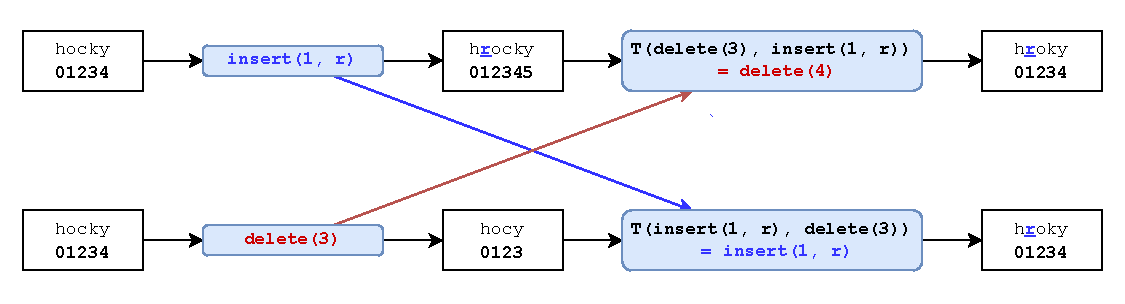
\includegraphics[scale=0.8]{figures/ot-transform}
    \caption[TP1 in action]{TP1 in action. Two sites start from \texttt{hocky}; one inserts \texttt{r} at index~1 while the other deletes index~3. Each site transforms the other's operation against its own, and both arrive at \texttt{hroky}.}
    \label{fig:OTschema}
\end{figure}

TP1 states that applying $\op_1$ and then $\op_2$ transformed against $\op_1$ gives the same document as applying $\op_2$ and then $\op_1$ transformed against $\op_2$ (Figure~\ref{fig:OTschema}). It matters whenever two operations reach two replicas in different orders. An OT algorithm that satisfies TP1 alone is enough to build a client-server system with a single source of truth. In OT systems that do not rely on TP2, convergence requires every operation to be transformed against one shared context~\citep{Xu2016}: for example, the history of operations held on the server can be treated as the authoritative order for every client~\citep{Vidot2000}. When a client receives new operations from the server, it transforms all of its local operations that the server has not yet accepted against them. The server accepts a client's operation only once the client already has every operation the server holds.

TP2 states that transforming a third operation $\op_3$ against $\op_1$ and $\op_2$ gives the same result whichever of the two equivalent orders they were applied in. It is needed only in systems that let two operations be executed on two different document states, that is, where concurrent operations are transformed at different sites rather than against one central history. Algorithms that satisfy TP2 are hard to get right: several published ones were later proven wrong~\citep{OTOverview1}. This difficulty is one reason CRDTs were introduced as an alternative to OT for keeping data consistent and correct across a distributed system.

\section{Conflict-Free Replicated Data Types (CRDTs)}
\label{sec:crdt}

In 2005, \citet{oster2005real} introduced WOOT (WithOut Operational Transformation), the first algorithm that makes the text replicas of a collaborative editor converge without OT. It also preserves the \emph{intention} of an operation, what the operation means to do~\citep{Li2004}. Take the string \texttt{ABCDE}, indexed from $0$, and suppose a client inserts the character \texttt{X} between \texttt{A} and \texttt{B}. The intention is to insert \texttt{X} so that \texttt{A} precedes \texttt{X} and \texttt{X} precedes \texttt{B}. In OT this insertion is written $\texttt{insert}(1, \texttt{X})$; in WOOT it is written $\texttt{insert}(\texttt{A} \prec \texttt{X} \prec \texttt{B})$, where \texttt{A} and \texttt{B} are objects with an identifier unique to each character in the string (Figure~\ref{fig:2:crdt-insert}). WOOT was the starting point for CRDTs, which \citet{Shapiro2011} formally defined in 2011, not only for strings but for many other abstract data types.

\begin{figure}[htbp]
    \centering
    % The same insertion in OT and in a CRDT: ABCDE, a client inserts X between
% A and B. Top: OT addresses characters by index. Bottom: a CRDT addresses
% them by ID, a (client, counter) pair, and keeps a deleted character as a
% tombstone. TikZ libraries: arrows.meta, positioning, fit, backgrounds.
% Colors from thesis.sty.
\begin{tikzpicture}[
  font=\sffamily\footnotesize,
  cell/.style={draw=black!60, line width=0.6pt, fill=white, minimum width=1cm,
    minimum height=0.6cm, inner sep=0pt, font=\ttfamily\small},
  obj/.style={draw=black!60, line width=0.6pt, fill=white, rounded corners=2pt,
    minimum width=0.7cm, minimum height=0.6cm, inner sep=0pt, font=\ttfamily\small},
  new/.style={draw=accent, fill=accentlight, text=accent, font=\ttfamily\small\bfseries},
  tomb/.style={draw=rulegray, fill=codebg, text=rulegray, dash pattern=on 2pt off 1.5pt},
  idx/.style={font=\sffamily\scriptsize, text=black!65, inner sep=1pt},
  oid/.style={font=\ttfamily\scriptsize, text=black!75, inner sep=1pt},
  link/.style={line width=0.6pt, black!60, -{Stealth[length=1.6mm,width=1.3mm]}},
  op/.style={line width=1pt, accent, -{Stealth[length=2.6mm,width=2mm]}},
  oplab/.style={above, font=\ttfamily\footnotesize, text=accent, inner sep=2pt},
  title/.style={font=\sffamily\small\bfseries, text=accent, anchor=west, inner sep=0pt},
  note/.style={font=\sffamily\footnotesize, text=black!70, inner sep=1pt},
  panel/.style={draw=rulegray, line width=0.6pt, rounded corners=3pt, inner sep=0.25cm},
  brace/.style={draw=black!45, line width=0.5pt},
]
  % Character centers: before at x = 0.5 + i, after at x = 8.9 + i.
  % ---- OT: by index ------------------------------------------------------
  \node[title] (t1) at (0,0) {OT: by index};
  \def\yr{-0.85}
  \foreach \ch [count=\i from 0] in {A,B,C,D,E} {
    \node[cell] (o\i) at ({0.5+\i},\yr) {\ch};
    \node[idx] at ({0.5+\i},\yr-0.52) {\i};
  }
  \draw[op] (5.3,\yr) -- node[oplab] {insert(1, X)} (8.1,\yr);
  \foreach \ch [count=\i from 0] in {A,X,B,C,D,E} {
    \ifnum\i=1 \node[cell, new] (p\i) at ({8.9+\i},\yr) {\ch};
    \else \node[cell] (p\i) at ({8.9+\i},\yr) {\ch}; \fi
  }
  \node[idx] at (8.9,\yr-0.52) {0};
  \node[idx, text=accent, font=\sffamily\scriptsize\bfseries] at (9.9,\yr-0.52) {1};
  \foreach \i in {2,...,5}
    \node[idx, text=accent, font=\sffamily\scriptsize\bfseries] at ({8.9+\i},\yr-0.52) {\i};
  % brace under the indices of B..E
  \def\yb{-1.62}
  \draw[brace] (10.5,\yb+0.08) -- (10.5,\yb) -- (14.3,\yb) -- (14.3,\yb+0.08);
  \draw[brace] (12.4,\yb) -- (12.4,\yb-0.08);
  \node[note, below] (n1) at (12.4,\yb-0.08) {B--E shift: each index $+1$};
  \begin{scope}[on background layer]
    \node[panel, fit=(t1)(o0)(p5)(n1)] {};
  \end{scope}

  % ---- CRDT: by identifier ----------------------------------------------
  \node[title] (t2) at (0,-2.75) {CRDT: by identifier};
  \node[note, anchor=west, text=black!60] at (t2.east) {\quad ID = \texttt{(client, counter)}};
  \def\yo{-4.1}
  \foreach \ch/\id [count=\i from 0] in {A/{1,1},B/{1,2},C/{1,3},D/{2,1},E/{2,2}} {
    \node[obj] (q\i) at ({0.5+\i},\yo) {\ch};
    \node[oid] at ({0.5+\i},\yo-0.52) {(\id)};
  }
  \foreach \i [evaluate=\i as \j using int(\i+1)] in {0,...,3}
    \draw[link] (q\i) -- (q\j);
  \draw[op] (5.3,\yo) -- node[oplab] {insert(A $\prec$ X $\prec$ B)} (8.1,\yo);
  % after: A X B C D E, with D deleted (a tombstone)
  \node[obj] (r0) at (8.9,\yo) {A};
  \node[obj, new] (r1) at (9.9,\yo) {X};
  \node[obj] (r2) at (10.9,\yo) {B};
  \node[obj] (r3) at (11.9,\yo) {C};
  \node[obj, tomb] (r4) at (12.9,\yo) {D};
  \node[obj] (r5) at (13.9,\yo) {E};
  \draw[rulegray, line width=0.8pt] ([xshift=-1.5mm]r4.center) -- ([xshift=1.5mm]r4.center);
  \foreach \i [evaluate=\i as \j using int(\i+1)] in {0,...,4}
    \draw[link] (r\i) -- (r\j);
  \node[oid] at (8.9,\yo-0.52) {(1,1)};
  \node[oid, text=accent, font=\ttfamily\scriptsize\bfseries] at (9.9,\yo-0.52) {(3,1)};
  \node[oid] at (10.9,\yo-0.52) {(1,2)};
  \node[oid] at (11.9,\yo-0.52) {(1,3)};
  \node[oid, text=rulegray] at (12.9,\yo-0.52) {(2,1)};
  \node[oid] at (13.9,\yo-0.52) {(2,2)};
  % X remembers its neighbors at insertion time
  \draw[accent, line width=0.6pt, -{Stealth[length=1.6mm,width=1.3mm]}]
    (r1.north) to[out=110, in=70] node[above, font=\sffamily\scriptsize, inner sep=1pt] {left} (r0.north);
  \draw[accent, line width=0.6pt, -{Stealth[length=1.6mm,width=1.3mm]}]
    (r1.north) to[out=70, in=110] node[above, font=\sffamily\scriptsize, inner sep=1pt] {right} (r2.north);
  \node[note, above=1pt of r4, text=black!60, align=center] (n3)
    {D, deleted by another user:\\[-1pt] kept as a tombstone};
  % brace under the IDs of B..E
  \def\yc{-4.87}
  \draw[brace] (10.5,\yc+0.08) -- (10.5,\yc) -- (14.3,\yc) -- (14.3,\yc+0.08);
  \draw[brace] (12.4,\yc) -- (12.4,\yc-0.08);
  \node[note, below] (n2) at (12.4,\yc-0.08) {B--E keep their IDs};
  \begin{scope}[on background layer]
    \node[panel, fit=(t2)(q0)(r5)(n2)(n3)] {};
  \end{scope}
\end{tikzpicture}%

    \caption[The same insertion in OT and in a CRDT]{The same insertion in OT and in a CRDT. OT addresses characters by index, so a concurrent edit can shift the index and the operation must be transformed. A CRDT gives every character a unique ID and inserts the new character between the IDs of its neighbors; a deleted character stays in the sequence as a tombstone.}
    \label{fig:2:crdt-insert}
\end{figure}

A CRDT is an abstract data type that keeps the replicas of a piece of data in agreement across a network. Being an abstract data type means that its semantics are defined by its values and by its operations, so different implementations can realize each operation differently yet behave the same. A CRDT is stored on every client or peer in the network, so memory- and time-efficient implementations matter. Each replica can be modified without coordinating with the others, and if every replica applies the same operations, in any order, they all reach the same final state~\citep{Shapiro2011, CRDToverview2}.

A simple example is a set. A grow-only set, which only supports \texttt{insert(v)}, is trivially a CRDT, because insertions commute. Supporting \texttt{erase(v)} as well needs a rule for an insertion and an erasure of the same element that happen concurrently, for example letting the insertion win, as an observed-remove set does~\citep{Shapiro2011}. In this study, CRDTs are used for text, so the operations involved are the same as in Section~\ref{subsec:OT}: \texttt{insert(pos, c)} and \texttt{delete(pos)}.

In a CRDT for plain text, every character has its own ID. An insertion carries, along with the new character, the IDs of the characters before and after it, and a logical clock that records the order of insertions, the same idea as in WOOT~\citep{oster2005real}. There are two common ways to handle deletion. The first keeps deleted characters in the document forever and only marks them as deleted, a technique known as a \emph{tombstone}~\citep{molli2006tombstone}. The second assigns IDs that are already ordered by position: a character inserted at a given position gets an ID greater than that of the character before it and smaller than that of the character after it. These IDs must be able to grow, so that there is always room for a new ID between two others, and each carries a further identifier unique to its client, so that no two IDs are ever the same. Because the order is in the IDs themselves, a deleted character does not need to be kept.

Compared with OT, which needs only its transformation functions and can represent the document as a plain array of characters, a CRDT needs an additional data structure for every character in the document. Each character gets an ID and becomes an object, linked, implicitly or explicitly, to the characters before and after it, as in the two approaches above.

\section{A Closer Comparison of CRDT and OT}
\label{sec:perbandingan}

Real-time collaborative text editors in industry are still dominated by operational transformation, even though CRDTs are claimed to have better complexity and efficiency~\citep{Sun2019third}. The line between the two is not sharp: at heart, both transform operations so that they commute, and they differ in the parameters they use. A CRDT converts an operation into a representation based on IDs, or other identifiers, and back into a position once it is applied; OT expresses an operation directly by the position of its characters.

OT centers on transformation algorithms that manage the concurrent operations of every client. CRDTs center on the content: the ordering of objects, identifier-based operations, and other representations of edits~\citep{Sun2019Second, Sun2019First}. Proving a CRDT correct is harder than proving an OT algorithm correct, because of the special treatment of its content state~\citep{Sun2019Second}. Every CRDT needs its own criteria to meet its consistency conditions, depending on how it stores its data, and CRDTs for different abstract data types, such as sets, maps and text, each have their own implementation, algorithm and representation. This variety makes convergence harder to prove for CRDTs than for OT, whose basic conditions were proven by earlier research, so that a new OT algorithm only needs to satisfy them~\citep{OTOverview1, Sun2004, oster2005real}.

The two approaches also differ in complexity. In OT, the cost depends on the number of concurrent operations, and nothing is spent on representing the characters of the text as objects. In a CRDT, the cost grows with the size of the document, and setting up a new peer that joins the network also tends to take more time and memory than in OT.

According to \citet{Sun2019Second}, a state-of-the-art OT system takes $O(c)$ time to apply a remote operation and $O(1)$ to apply a local one, with a memory complexity of $O(c)$ or $O(c \cdot m)$, where $c$ is the number of concurrent operations to be transformed and $m$ is the number of users in the network. In practice $c$ is very small ($c \leq 10$), because operations happen in real time, and $m$ is usually at most $5$.

In the same analysis, define $C$ as the size of the content without tombstones, and $C_t$ as the content over the document's whole lifetime, tombstones included. The time complexity of a CRDT operation ranges from $O(C_{t}^{2})$ and $O(C_{t})$ down to $O(1)$ for tombstone-based CRDTs, and is $O(\log C)$ for solutions without tombstones. Memory can be brought down to $O(C)$, both without tombstones and with tombstones plus garbage collection. For typical documents, $10^3 \leq C \leq 10^6$.

\section{Related Work}
\label{sec:penelitian_terkait}

This study uses the Yjs library, which implements the YATA (Yet Another Transformation Approach) CRDT~\citep{Nicolaescu2016yjs}. YATA represents a document as a linked list of objects and uses tombstones, with a garbage collector that cleans up the content of objects marked as deleted. An insertion adds an object \texttt{o(id, left, right, isDeleted, content)} to the list. The \texttt{id} is a pair of the peer's ID and a logical timestamp, the number of operations that peer has performed so far. The fields \texttt{left} and \texttt{right} hold the \texttt{id}s of the objects to the left and to the right of the insertion at the time it was made. The boolean \texttt{isDeleted} records whether the object has been deleted, so the editor knows whether to show it, and \texttt{content} holds the object's data.

Yjs's main optimization is in \texttt{content}, which can hold a whole run of characters rather than one. When an insertion falls inside the content of an existing object, that object is split in two, so each object also stores the length of its content. A deletion simply marks the object as deleted. \citet{Nicolaescu2016yjs} give further details of the implementation and its compression. To synchronize, Yjs peers summarize what they have seen as a \emph{state vector}: the latest logical timestamp received from each peer in the network.

Yjs gained popularity in the few years before this study, and other sequence CRDTs have also been implemented. In Logoot, each object's position identifier combines a position with the ID of the site that created it and that site's logical clock, and a deletion removes the object directly, without leaving a tombstone~\citep{weiss2009logoot}. LSEQ refines how such position identifiers are allocated~\citep{nedelec2013lseq}. Position-based CRDTs like these can suffer from \emph{interleaving}: when two users concurrently type text at the same place, their characters can end up interleaved with each other, rather than kept as two separate runs~\citep{kleppmann2019interleaving}. YATA orders concurrent insertions that share the same neighbors with a deterministic rule based on the IDs of the clients that made them~\citep{Nicolaescu2016yjs}.

RGA (Replicated Growable Array) is an alternative to YATA~\citep{roh2011replicatedrga}. It orders concurrent insertions with a pair of the peer's ID and a logical timestamp greater than any timestamp the peer has seen. In practice, implementations of these algorithms add many optimizations beyond the formal algorithms in their papers, such as garbage collection, compression of the data sent over the network, and the way objects are laid out in memory, and these affect their performance.
